\documentclass[10pt,twocolumn]{article}

\usepackage[margin=0.82in,columnsep=0.25in]{geometry}
\usepackage[T1]{fontenc}
\usepackage[utf8]{inputenc}
\usepackage{lmodern}
\usepackage{microtype}
\usepackage{graphicx}
\usepackage{booktabs}
\usepackage{tabularx}
\usepackage{array}
\usepackage{amsmath,amssymb}
\usepackage{enumitem}
\usepackage{caption}
\usepackage{subcaption}
\usepackage{xcolor}
\usepackage{url}
\usepackage[hidelinks]{hyperref}
\hypersetup{
  pdftitle={Facial-Expression Classification on FER2013: Comparing an MLP and a CNN},
  pdfauthor={Satya Siddhartha Balanagu},
  pdfsubject={Assignment 1 technical report},
  pdfkeywords={FER2013, facial expression recognition, CNN, education research}
}

\graphicspath{{figures/}}
\captionsetup{font=small,labelfont=bf}
\setlist{nosep,leftmargin=*}
\setlength{\parindent}{1em}
\setlength{\parskip}{0pt}
\renewcommand{\arraystretch}{1.08}
\makeatletter
\setlength{\@fptop}{0pt}
\setlength{\@dblfptop}{0pt}
\makeatother

\newcolumntype{Y}{>{\raggedright\arraybackslash}X}
\newcommand{\task}[1]{\section{Task #1}}

\title{\textbf{Facial-Expression Classification on FER2013:}\\
\large Comparing an MLP and a CNN}

\author{
Satya Siddhartha Balanagu\\
Student ID: A1961325\\
University of Adelaide
}

\date{28 August 2026}

\begin{document}
\raggedbottom
\maketitle

\begin{abstract}
This study compares an MLP with a CNN for seven-class facial-expression classification. The supplied data contain 35,887 FER2013 images, not FER+ relabelled data. The official Training partition supplied the training and validation sets, while PublicTest was reserved for final testing. Each model received the same 15-epoch budget and training-only augmentation. The MLP reached 37.7\% accuracy and 0.247 macro-F1. The CNN reached 54.4\% accuracy and 0.430 macro-F1, but it failed to identify any of the 56 Disgust test images. The CNN is the stronger research baseline, not a system for classroom decisions. FER2013 has no demographic data, and a face image cannot establish a person's internal emotional state.
\end{abstract}

\noindent\textbf{Keywords:} FER2013, facial expression recognition, convolutional neural network, education research, model evaluation

\task{1: Data Exploration and Preprocessing}

\subsection{Dataset Identification and Scope}

FER2013 was introduced for the 2013 facial-expression recognition challenge~\cite{goodfellow2013}. Each CSV row contains an integer emotion label, a string of 2,304 grayscale pixel values, and a predefined usage split. The pixels form a $48\times48$ image. The seven labels are Angry (0), Disgust (1), Fear (2), Happy (3), Sad (4), Surprise (5), and Neutral (6).

The local archive was downloaded on 25 August 2026 from the Kaggle FER2013 repository by deadskull7~\cite{fer2013kaggle}: \url{https://www.kaggle.com/datasets/deadskull7/fer2013}. The supplied file is retained as \texttt{fer2013.csv}; the archive is the original FER2013 release rather than FER+.

The local archive contains \texttt{fer2013.csv}; it does not contain the crowd-sourced label distributions that define FER+~\cite{barsoum2016}. The analysis therefore uses the name FER2013 throughout. In the education-research setting considered here, the labels are used only as visible expression categories, not as measurements of learning or internal emotional state.

The labels also limit the conclusion that can be drawn. FER2013 supplies one hard category per image, whereas FER+ records disagreement between annotators. The models can be compared on this benchmark, but the scores do not show that either model has recovered a person's true emotional state.

The CSV has 35,887 rows and three columns. No missing values were found, and every pixel string contains exactly 2,304 values. The predefined usage counts are 28,709 Training, 3,589 PublicTest, and 3,589 PrivateTest images.

\begin{table}[t]
\centering
\caption{FER2013 class distribution.}
\label{tab:classes}
\begin{tabular}{lrr}
\toprule
Class & Images & Share \\
\midrule
Angry & 4,953 & 13.8\% \\
Disgust & 547 & 1.5\% \\
Fear & 5,121 & 14.3\% \\
Happy & 8,989 & 25.0\% \\
Sad & 6,077 & 16.9\% \\
Surprise & 4,002 & 11.2\% \\
Neutral & 6,198 & 17.3\% \\
\bottomrule
\end{tabular}
\end{table}

\subsection{Exploratory Data Analysis}

Table~\ref{tab:classes} and Fig.~\ref{fig:distribution} show a strong imbalance. Happy has 8,989 images, compared with 547 for Disgust. Accuracy alone may hide failure on the smaller classes, so the evaluation also reports macro-averaged precision, recall, and F1.

The imbalance is a modelling issue, not just a property of the dataset. A classifier can increase accuracy by favouring frequent classes, even if it rarely predicts Disgust or Fear. Disgust has roughly one-sixteenth as many examples as Happy, so a few correct or incorrect predictions can change its class-level score substantially. Reporting macro metrics alongside accuracy makes that trade-off visible by giving each class equal weight in the average.

\begin{figure*}[t]
\centering
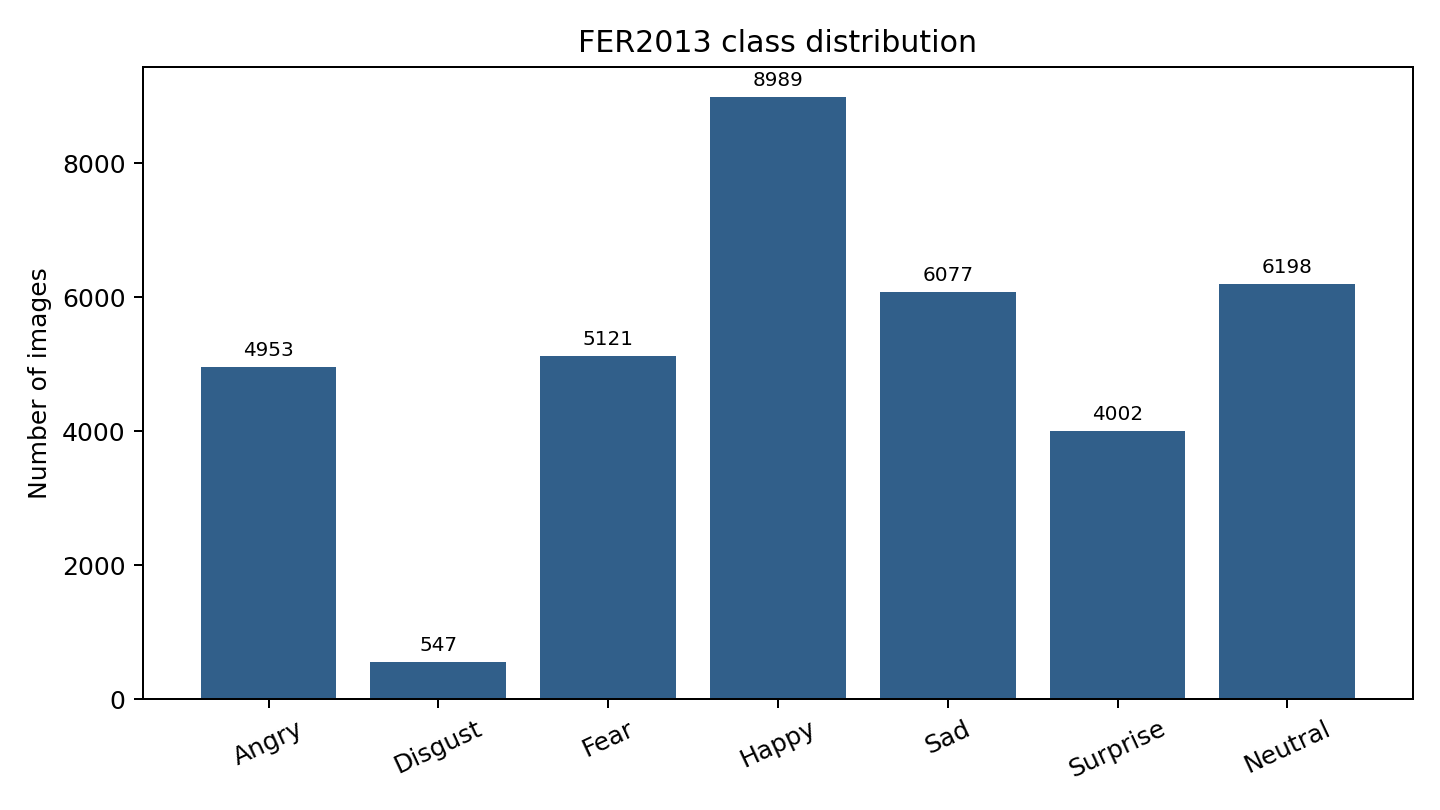
\includegraphics[width=0.68\textwidth]{class_distribution.png}
\caption{Full FER2013 class distribution. Disgust is severely under-represented, while Happy forms one quarter of the dataset.}
\label{fig:distribution}
\end{figure*}

The examples in Fig.~\ref{fig:samples} show why this is a difficult dataset. The images are small and inconsistently framed. Lighting, head position, obstructions, and expression strength also vary. Some labels are visually ambiguous, and the missing context means that an image labelled ``sad'' or ``angry'' cannot establish the person's actual emotional state~\cite{barrett2019}. The sample grid and the class-wise mean images are descriptive EDA computed from the full CSV, including PublicTest and PrivateTest.

\begin{figure*}[t]
\centering
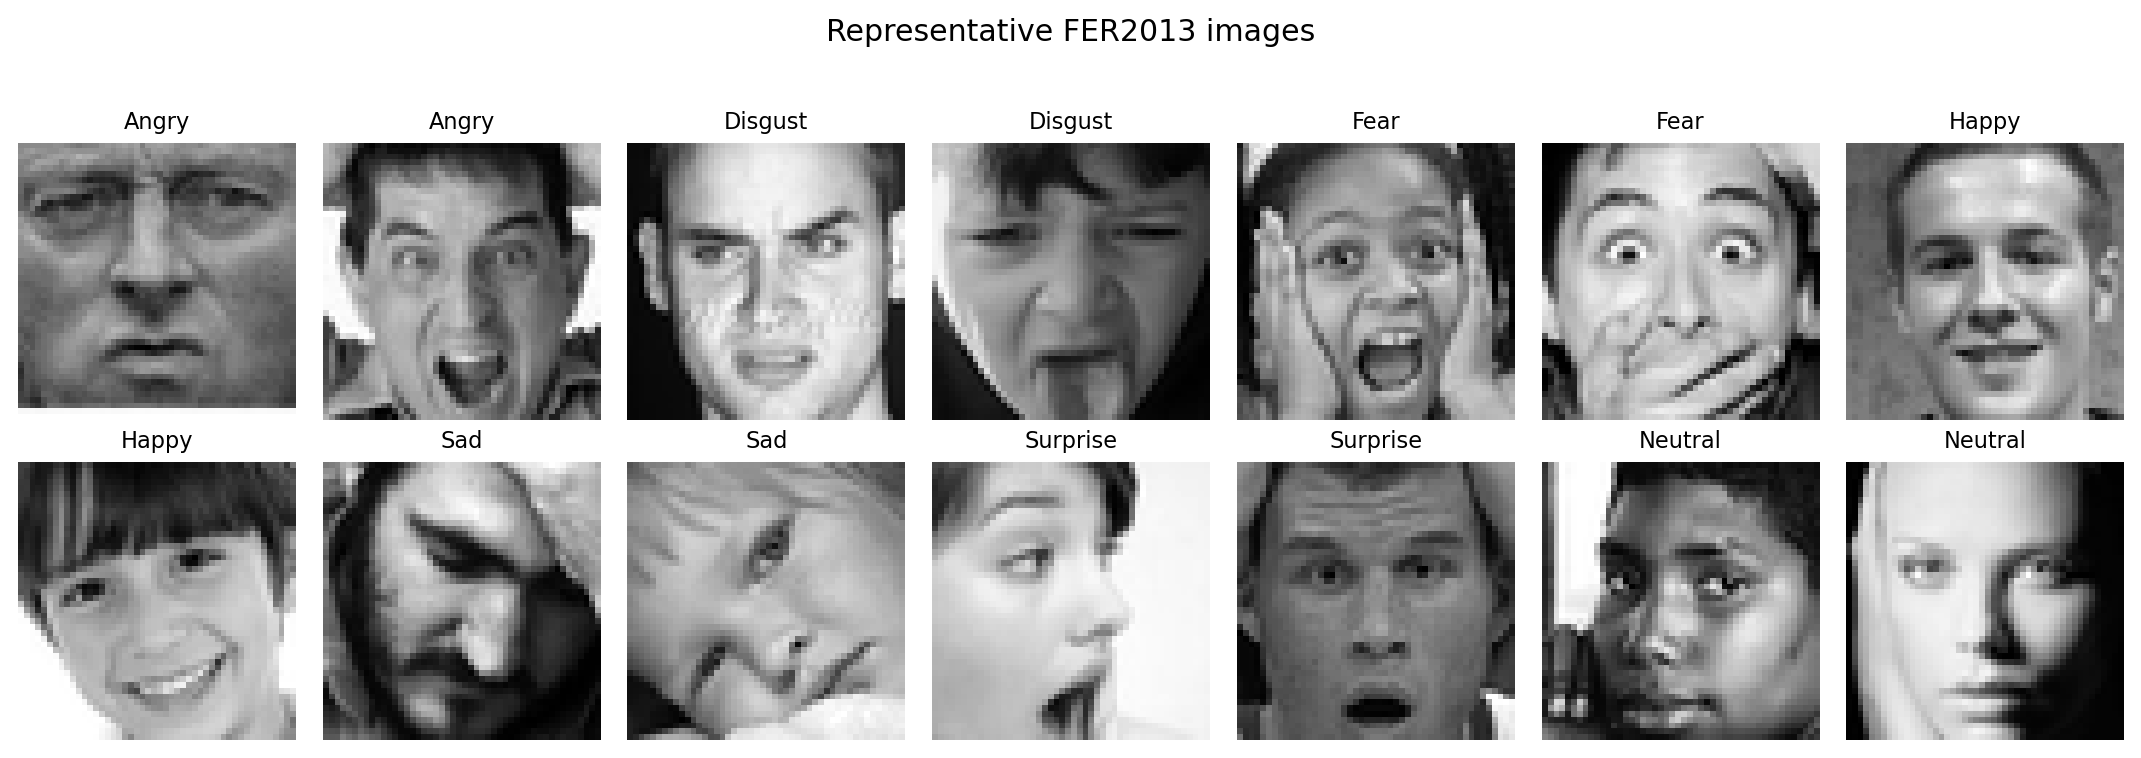
\includegraphics[width=0.94\textwidth]{sample_grid.png}
\caption{Two representative images per FER2013 class. Variation and ambiguity are visible even within a small sample.}
\label{fig:samples}
\end{figure*}

Class-wise mean images provide a second EDA view beyond the count statistics and individual examples (Fig.~\ref{fig:means}). The averages are diffuse, so they describe aggregate pixel structure rather than canonical emotional appearances.

\begin{figure*}[t]
\centering
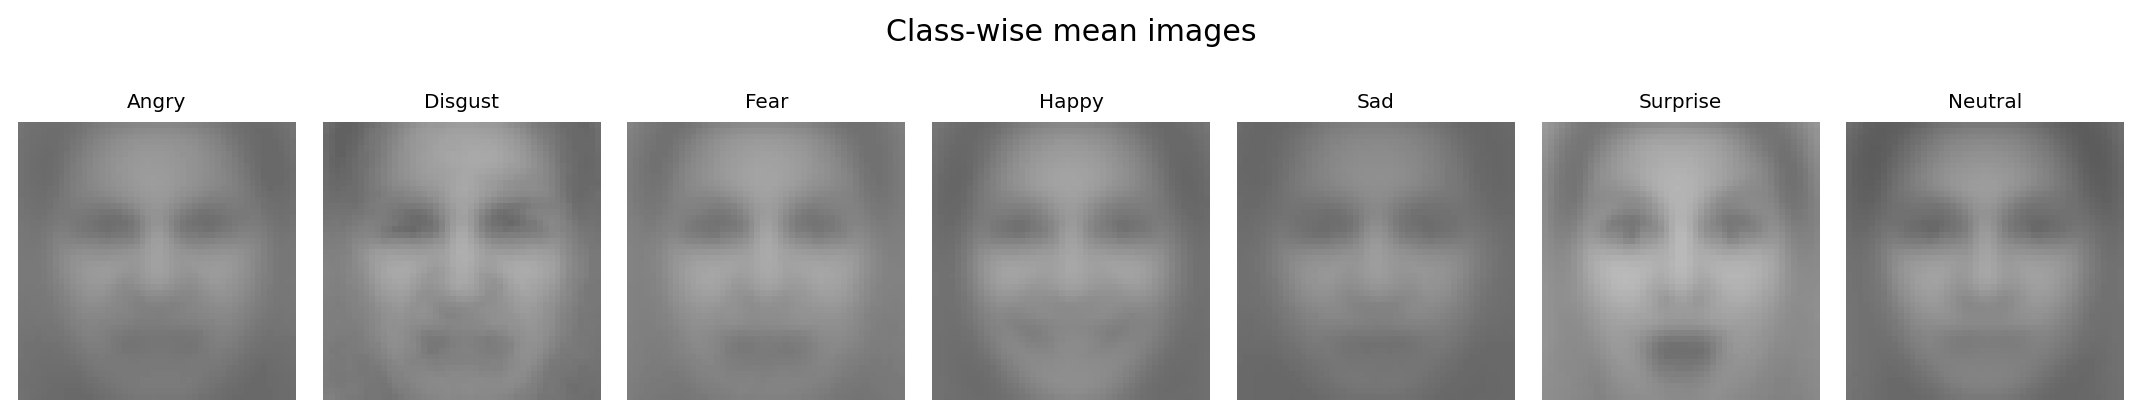
\includegraphics[width=0.94\textwidth]{class_mean_images.png}
\caption{Class-wise mean images computed from all FER2013 examples. The diffuse averages reflect variation within each label.}
\label{fig:means}
\end{figure*}

\subsection{Preprocessing and Split Design}

Pixel strings were parsed as unsigned 8-bit values, reshaped to $1\times48\times48$, and scaled from $[0,255]$ to $[0,1]$. Scaling keeps the input magnitude consistent with the optimisation settings and avoids giving the raw 8-bit range an unnecessarily large influence on the first layer. All rows passed the schema and pixel-count checks, so none were removed. Resizing was unnecessary because every image is already $48\times48$; resizing would add an interpolation step without adding information. The CNN received the normalised image tensor directly, while the same values were flattened for the MLP baseline so that the input representation was otherwise held constant.

Using seed 42, the official Training partition was divided by a stratified split into 25,835 training images and 2,874 validation images. A 90/10 split preserves most examples for fitting while leaving enough validation images to compare all seven classes. Stratification prevents the rare classes from disappearing from the validation set or being represented at very different rates. PublicTest and PrivateTest were excluded from training and checkpoint selection. PublicTest was evaluated only after model selection, while PrivateTest was not used for performance evaluation. During training, images could be flipped horizontally with probability 0.5 or rotated by up to $10^{\circ}$. Validation and test images were left unchanged. Both models used the same stochastic augmentation policy, but independent training passes can receive different random transformations. The transformations represent small changes in pose and alignment; they do not create new demographic coverage or correct the class imbalance.

\task{2: Model Selection and Training}

\subsection{Learning Task and Model Rationale}

The task is supervised multiclass image classification. Two models were chosen to isolate the value of spatial structure.

\textbf{MLP baseline.} Each image is flattened to 2,304 values, followed by 128 ReLU units, dropout with $p=0.25$, and seven output logits. This baseline provides a simple test of what happens when neighbouring pixels are not modelled explicitly. Once flattened, a pixel's location is still encoded by its input position, but the network must learn relationships between distant positions without the local weight sharing used by a CNN. The single hidden layer keeps the baseline inexpensive and interpretable, while dropout limits reliance on individual hidden units. It is not intended as a strongest-possible classical vision baseline.

\textbf{CNN.} The CNN has three convolutional blocks with 32, 64, and 128 channels, followed by a 128-unit dense layer. Each block combines convolution with batch normalisation, ReLU, pooling, and dropout. Early convolutional layers can represent local edges and intensity changes; later layers combine these into larger facial patterns as pooling reduces spatial resolution. Increasing the channel count as the feature maps become smaller gives later layers more feature types to combine. Local receptive fields and shared weights preserve image structure~\cite{lecun1998}, allowing the network to learn spatial features without hand-crafted landmarks or texture descriptors.

Table~\ref{tab:models} lists the two configurations and their intended roles. The MLP has 295,943 trainable parameters, whereas the CNN has 730,151; the comparison therefore also reflects model capacity.

\begin{table*}[t]
\centering
\caption{Model configurations.}
\label{tab:models}
\begin{tabularx}{\textwidth}{lYl}
\toprule
Model & Architecture & Purpose \\
\midrule
MLP & Flatten $\rightarrow$ 128 ReLU $\rightarrow$ dropout 0.25 $\rightarrow$ 7 logits & Non-convolutional baseline \\
CNN & Conv blocks 32/64/128 $\rightarrow$ pooling and dropout $\rightarrow$ 128 ReLU $\rightarrow$ 7 logits & Learn local spatial features \\
\bottomrule
\end{tabularx}
\end{table*}

\subsection{Training Procedure}

Both models were implemented in PyTorch~\cite{paszke2019} and trained on the Apple MPS backend. Multiclass cross-entropy was minimised with Adam~\cite{kingma2015}, learning rate $8\times10^{-4}$, and weight decay $10^{-4}$. Adam supplies adaptive parameter updates for the two models, while weight decay provides a small regularising pressure. Batch sizes were 128 for training and 256 for validation and testing. A cosine learning-rate schedule reduced the step size across training, allowing larger updates early and smaller updates as the fixed budget approached its end.

Both models used the same split and stochastic augmentation pipeline. The CNN contains approximately 730,151 trainable parameters compared with 295,943 for the MLP. The comparison therefore measures the practical benefit of the complete CNN design, not spatial structure alone.

Each model ran for 15 epochs. After every epoch, validation macro-F1 was calculated and the best parameter state was retained. Macro-F1 was used for checkpoint selection because an accuracy-only rule could prefer a checkpoint that improves frequent classes while neglecting the rare classes. Epoch 14 was selected for the MLP and epoch 10 for the CNN before PublicTest was evaluated. Figure~\ref{fig:curves} shows the training record. The CNN validation loss was still falling slightly near the end, so this is a fixed-budget comparison rather than evidence of full convergence.

\begin{figure*}[t]
\centering
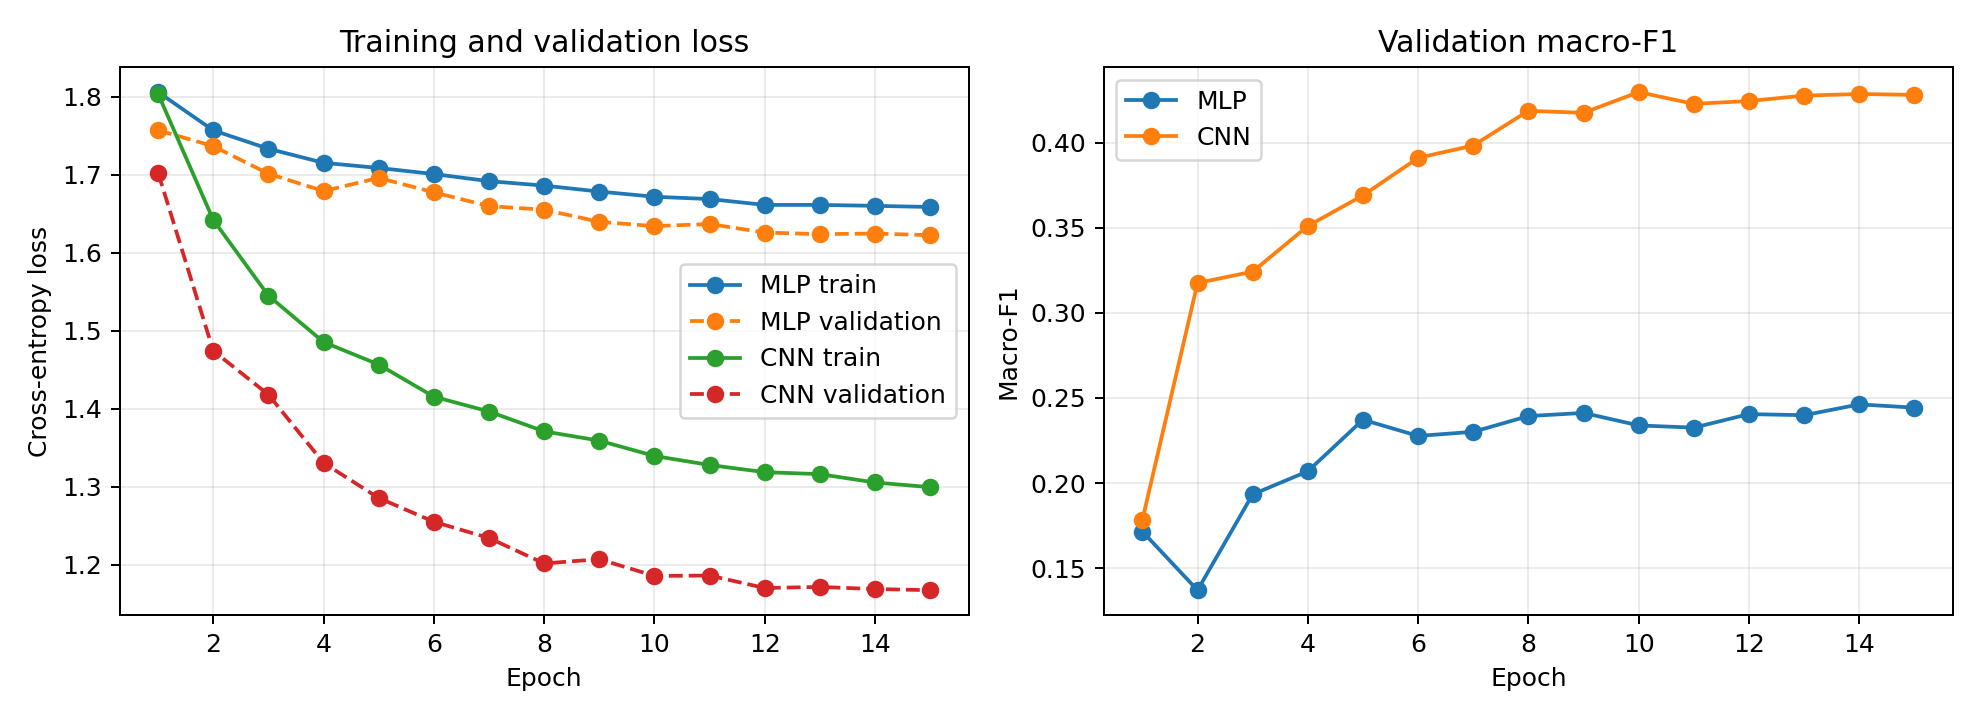
\includegraphics[width=0.88\textwidth]{training_curves.png}
\caption{Training and validation loss (left) and validation macro-F1 (right). The selected checkpoint is based only on validation macro-F1.}
\label{fig:curves}
\end{figure*}

\task{3: Model Evaluation and Interpretation}

\subsection{Evaluation Measures}

Accuracy measures the fraction of correct predictions but can hide minority-class failure. Precision measures how often a predicted class is correct, recall measures how much of the true class is recovered, and F1 is their harmonic mean. Macro averages weight all seven classes equally; weighted-F1 reflects class frequency. Confusion matrices expose specific error directions.

These measures answer different questions. Macro-F1 is the primary summary here because it gives the rare Disgust class the same weight as Happy. Weighted-F1 describes performance on the observed test mix, while accuracy gives the simplest count of correct predictions. Reading them together shows whether a model's average score depends mainly on the larger classes.

\subsection{Overall Results}

Table~\ref{tab:metrics} gives the PublicTest results. The CNN improves accuracy by 16.7 percentage points over the MLP, from 37.7\% to 54.4\%, and raises macro-F1 from 0.247 to 0.430. For context, always predicting Happy would score about 25.0\% accuracy. The MLP is only modestly above that baseline; the CNN separates more of the classes.

\begin{table}[t]
\centering
\caption{PublicTest performance.}
\label{tab:metrics}
\resizebox{\columnwidth}{!}{%
\begin{tabular}{lccccc}
\toprule
Model & Acc. & Macro-P & Macro-R & Macro-F1 & W-F1 \\
\midrule
MLP & 0.377 & 0.277 & 0.286 & 0.247 & 0.312 \\
CNN & \textbf{0.544} & \textbf{0.434} & \textbf{0.447} & \textbf{0.430} & \textbf{0.519} \\
\bottomrule
\end{tabular}}
\end{table}

The CNN's weighted-F1 is 0.519, compared with a macro-F1 of 0.430. The MLP has the same gap: 0.312 weighted-F1 against 0.247 macro-F1. Both models therefore perform better on the larger classes.

The CNN's weighted-F1 is useful for describing the observed test mix, but the lower macro-F1 shows that performance is still uneven across classes. The MLP's lower scores and stronger dependence on frequent classes make it a useful baseline, not a convincing solution for the image task.

\subsection{Class-Level Error Analysis}

Table~\ref{tab:perclass} shows the strongest CNN results for Happy (F1 0.782) and Surprise (0.708). Neutral reaches 0.530, while Angry and Sad remain near 0.4. Fear falls to 0.169. None of the 56 Disgust images is classified correctly, leaving precision, recall, and F1 at zero. Fear recall is only 0.113, meaning that most true Fear examples are missed even though the class has many more examples than Disgust. This pattern indicates that the CNN has learned useful separation for some visible configurations, but not a reliable representation for every label.
\begin{table}[t]
\centering
\caption{CNN class-level PublicTest metrics.}
\label{tab:perclass}
\begin{tabular}{lrrrr}
\toprule
Class & Precision & Recall & F1 & $n$ \\
\midrule
Angry & 0.437 & 0.362 & 0.396 & 467 \\
Disgust & 0.000 & 0.000 & 0.000 & 56 \\
Fear & 0.335 & 0.113 & 0.169 & 496 \\
Happy & 0.738 & 0.832 & 0.782 & 895 \\
Sad & 0.375 & 0.489 & 0.424 & 653 \\
Surprise & 0.658 & 0.766 & 0.708 & 415 \\
Neutral & 0.498 & 0.567 & 0.530 & 607 \\
\bottomrule
\end{tabular}
\end{table}

Figures~\ref{fig:cm-mlp} and~\ref{fig:cm-cnn} show the normalised confusion matrices. The MLP predicts mostly Happy, Sad, Surprise, or Neutral. The CNN uses more of the label set, but Sad remains a common destination for Angry, Fear, and Neutral images. Fear is confused with several classes rather than one consistent alternative.
The CNN confusion matrix explains why the overall accuracy needs caution. Disgust has no predicted instances, so the model does not cover all seven categories. Fear is distributed across Angry, Happy, Sad, Surprise, and Neutral rather than collapsing into one alternative, which is consistent with ambiguous facial configurations and the lack of contextual information. The matrix describes prediction behaviour, not the actual feelings of the people in the images.

\begin{figure}[!htbp]
\centering

\begin{subfigure}[t]{0.95\linewidth}
    \centering
    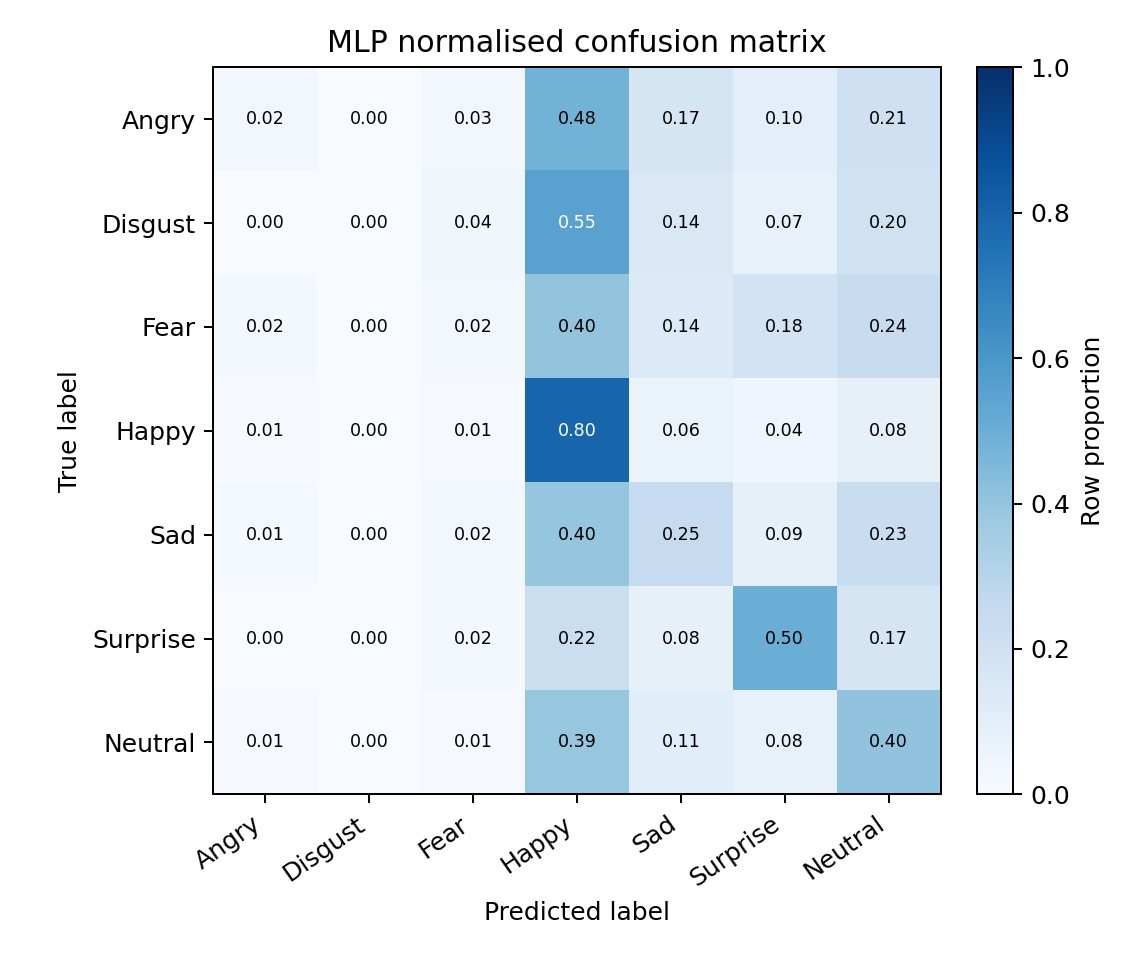
\includegraphics[width=\linewidth]{confusion_matrix_mlp.png}
    \caption{MLP normalised confusion matrix.}
    \label{fig:cm-mlp}
\end{subfigure}

\par\smallskip

\begin{subfigure}[t]{0.95\linewidth}
    \centering
    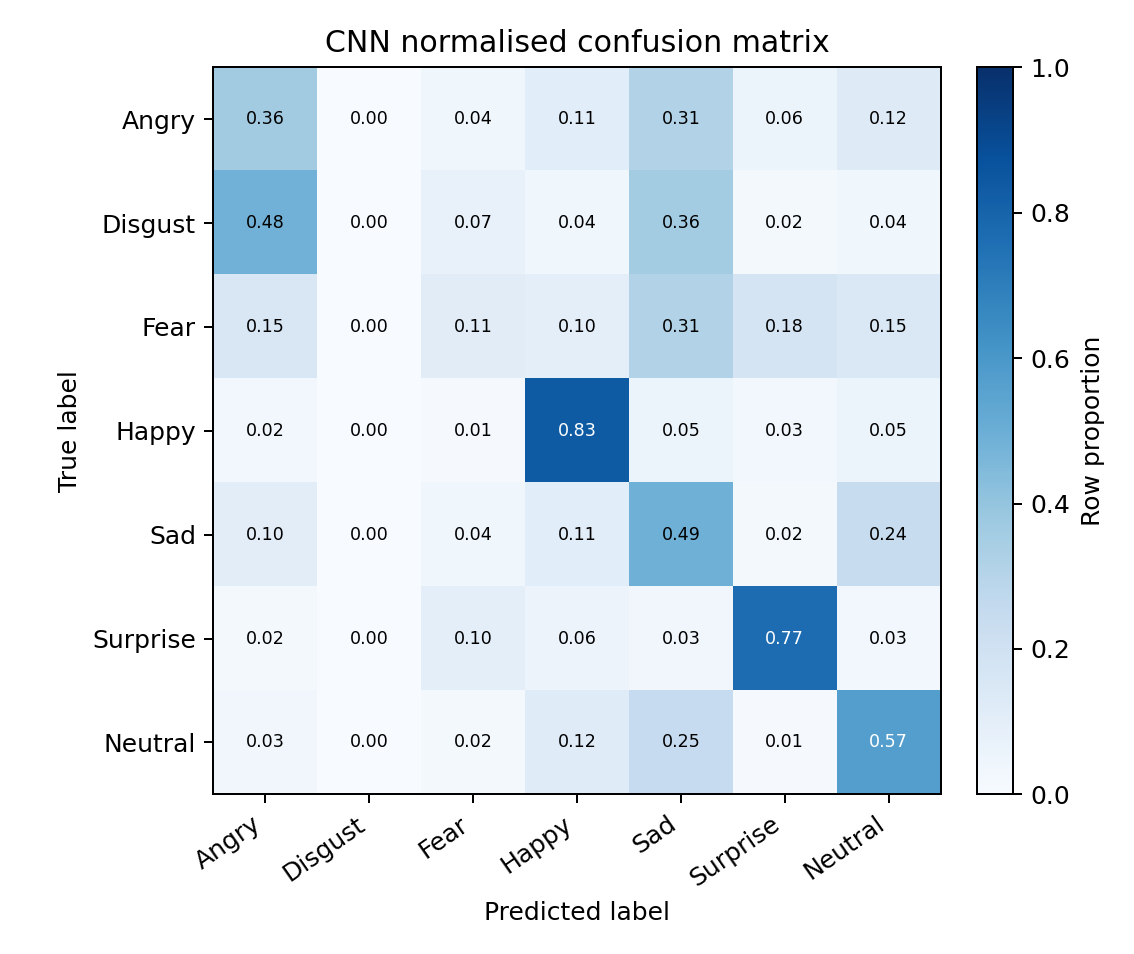
\includegraphics[width=\linewidth]{confusion_matrix_cnn.png}
    \caption{CNN normalised confusion matrix.}
    \label{fig:cm-cnn}
\end{subfigure}

\caption{Class-level error patterns. Rows are true classes and columns are predicted classes.}
\label{fig:confusions}
\end{figure}

Figure~\ref{fig:misclassifications} shows eight CNN errors from PublicTest, including repeated Fear--Sad and Sad--Neutral confusions. At this resolution, similar mouth, brow, and eye shapes appear under different labels. Tight crops remove further context. The examples show ambiguity in the dataset, not the cause of any person's emotion.

\begin{figure*}[t]
\centering
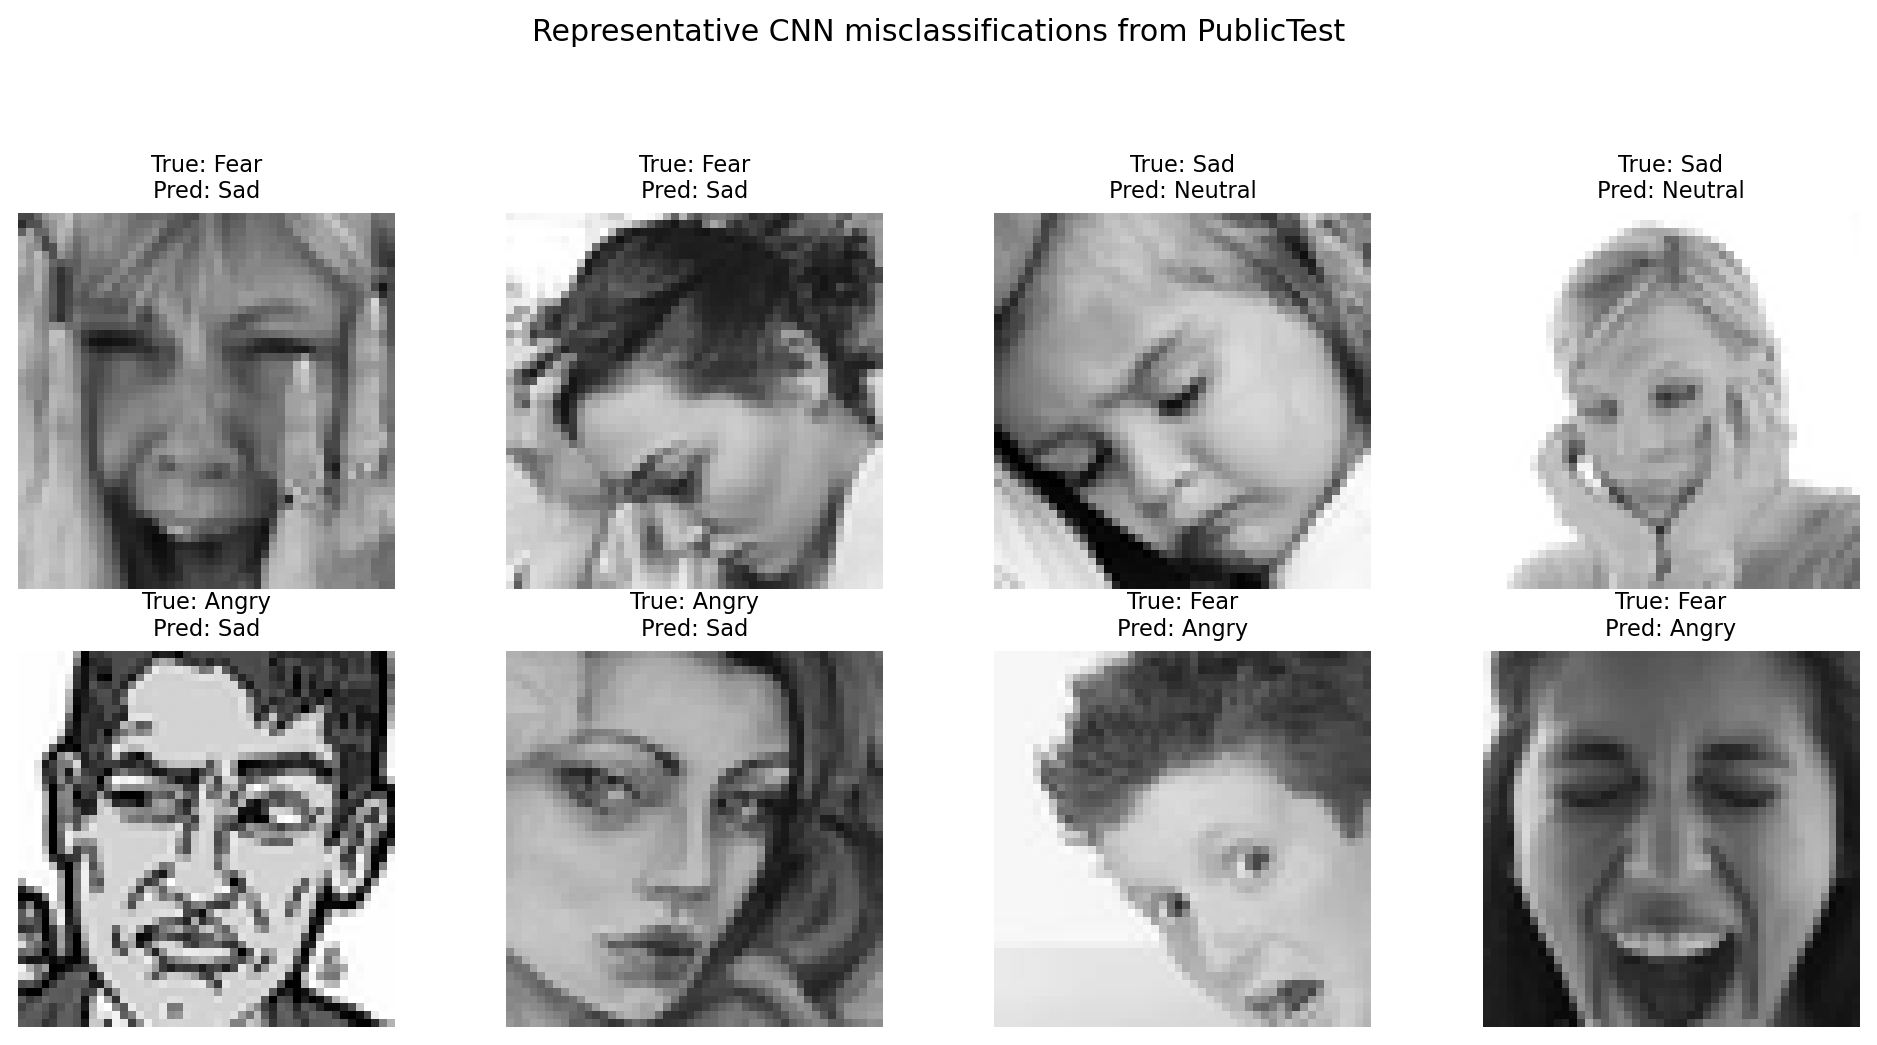
\includegraphics[width=1\textwidth]{misclassification_grid.png}
\caption{Eight selected CNN errors from PublicTest. Each title gives the dataset label and model prediction.}
\label{fig:misclassifications}
\end{figure*}

\subsection{Recommendation and Practical Implications}

The CNN is the better of the two tested models, but it is not ready for practical use. It misclassifies 45.6\% of PublicTest and fails completely on one class.

At most, it could support an opt-in study of aggregate expression-category counts under human supervision. It should not influence grades, discipline, attendance, wellbeing decisions, or claims about an individual student's engagement. Any later study would first need representative local data and independent validation. Subgroup testing, calibrated probabilities, an abstention option, and human review would also be required; none was evaluated here.

The restriction is a direct response to these errors. An individual-facing system would convert an uncertain category into a consequential judgement, while an aggregate research summary can be checked, challenged, and withheld when coverage is poor. Even the aggregate use would need a predefined purpose, opt-out route, retention limit, and a rule for stopping the study when minority-class or subgroup performance is inadequate.


\task{4: Ethical Considerations and Discussion}

\subsection{How Domain and Modality Shaped Decisions}

The image format favours convolution, while the education setting raises a different question: what harm could follow from an error? Students may have little practical freedom to refuse monitoring, and a false inference could change how they are treated. High aggregate accuracy would not remove the need for strict limits on purpose, careful data handling, and human responsibility.

The prediction target is narrower than the language often used around emotion-recognition systems. A camera records a face, but the model is trained on a human-assigned expression category, not on a direct measurement of emotion, attention, engagement, or wellbeing. The same visible movement can have different causes, and a neutral-looking face can occur during many different internal states. Treating the output as a psychological measurement would add an unsupported inference between the image and the decision.

The MLP is best treated as a low-cost educational or exploratory baseline. The CNN is more suitable for a carefully controlled, opt-in aggregate research study with human oversight, but neither model should make an individual educational decision. The CNN's stronger score does not change that boundary.

\subsection{Specific Risks and Mitigations}

The main risks arise from collecting identifiable faces in a setting with unequal power, then attaching psychological meaning to an unreliable label. Bias cannot be checked by demographic group, and the data could later be reused for surveillance or discipline. Table~\ref{tab:ethics} links these problems to basic controls.

Disgust makes up only 1.5\% of FER2013, and the CNN does not correctly classify any Disgust image in PublicTest. An aggregate classroom summary could therefore look acceptable while omitting a small class altogether. The wider pattern of errors also shows why facial movement is an unsafe proxy for a student's internal state.

\begin{table}[!htbp]
\centering
\caption{Ethical risks and practical mitigations.}
\label{tab:ethics}
\footnotesize
\begin{tabularx}{\columnwidth}{>{\raggedright\arraybackslash}p{1.82cm}Y}
\toprule
Risk & Minimum control \\
\midrule
Consent and privacy & Explicit, informed, revocable opt-in; non-participation path; data minimisation; encryption; prompt deletion of raw images. \\
Demographic and cultural bias & Representative evaluation data; subgroup metrics; independent review; suspend use when parity cannot be demonstrated. \\
Invalid inference & Expression-category wording only; no psychological or behavioural conclusions; contextual human review~\cite{barrett2019}. \\
Class imbalance & More minority examples; balanced methods; macro metrics; minimum per-class thresholds. \\
Function creep & Written purpose; role-based access; audit logs; retention limits; renewed approval for every new use. \\
\bottomrule
\end{tabularx}
\end{table}

Australian deployments should be reviewed against the Australian Privacy Principles. Current OAIC guidance states that collection must be reasonably necessary and that sensitive information generally requires consent~\cite{oaic2026}. In the European Union, GDPR imposes additional requirements; facial images processed to uniquely identify a person are biometric data under Article 4, and Article 9 applies special-category protections~\cite{gdpr2016}. This experiment classifies expressions rather than identity, but identifiable facial images still require careful privacy governance.

\subsection{Bias, Fairness, and Improvement}

FER2013 supplies no demographic labels, so subgroup performance cannot be checked. A later study would need consented local data with enough cases to estimate error rates for relevant groups and their intersections. Similar scores between groups would still not prove that inferring emotion from a face is valid.

Without demographic labels, this experiment cannot show whether errors are concentrated by skin tone, age, gender, disability, culture, lighting condition, or their intersections. Reweighting the existing classes would not repair that missing information. A responsible follow-up would need to define the relevant groups before collection, document how labels were obtained, and report uncertainty around subgroup metrics rather than treating a small sample as proof of parity.

The reported comparison used ordinary cross-entropy. Class weighting or balanced sampling should be tested because Disgust is rare, and a longer schedule may improve the CNN. Transfer learning and FER+ label distributions are further options. Better scores would not remove the underlying problem: facial movements have many-to-many relationships with emotion categories~\cite{barrett2019}.

\section{Limitations and Conclusion}

This is a small, single-seed comparison on one dataset. The 15-epoch limit was a shared training budget, not a convergence study, and only a narrow hyperparameter range was tried. PublicTest was evaluated once; PrivateTest remained unused. No confidence intervals, significance test, probability calibration, demographic audit, or classroom validation was produced. The parameter-count difference means the result does not isolate spatial structure from capacity, and a single run does not show how stable the ranking is across initialisations. FER2013 also assigns one label per image, whereas FER+ better represents disagreement between annotators~\cite{barsoum2016}.

The CNN is clearly stronger than the MLP on this benchmark. It raises accuracy from 37.7\% to 54.4\% and macro-F1 from 0.247 to 0.430, which is consistent with convolution preserving local image structure. That makes the CNN the better starting point for another experiment, but it does not justify classroom deployment while minority-class failure and label ambiguity remain unresolved.

\begingroup
\bibliographystyle{unsrt}
\bibliography{fer2013_references}
\endgroup

\end{document}
